%   MSc Business Analytics Dissertation
%   Format based on skeleton template provided as part of module MIS40750
%
%   Title:     Optimising the design of buffer preparation in bioprocessing
%              facilities
%   Author:    Sean Tully
%
%   Chapter 3: Data
%
%   Change Control:
%   When     Who   Ver  What
%   -------  ----  ---  --------------------------------------------------------
%   06Jun16  ST    0.1  Begun
%

\chapter{Data}\label{C.data}

\begin{quote}
We have some freedom in setting up our personal standards of beauty, but it is
especially nice when the things we regard as beautiful are also regarded by
other people as useful.

\hspace{2cm}--- Donald Knuth, \emph{Computer Programming as an Art}
\end{quote}

\section{Introduction}\label{S.intro3}

This section will outline what the input data might look like, including data
sources.
It will outline what form the output data and metrics should take.

For modelling a single process, a typical data-set consists of three distinct
files.
The first file is a table of data relating to the available selection of
vessels.
The second file is a table of data relating to parameters specific
to each buffer.
The third file comprises a collection of global parameters
that apply to all vessels and/or buffers.

One particular example, which is based on obfuscated data from a large-scale
facility, is used throughout this chapter to illustrate the format of the data.

\section{Vessel Data}\label{S.vesseldata}

\begin{table}[h!]
    \centering
    \caption{Vessel data for large-scale example}
    \label{tbl.vessel}
    \begin{tabular}{l | r | r}
        names & volumes & costs\\
        & $V_{m}$ (l) & $c_{m}$ (--)\\\hline
        \SI{2000}{\litre} & \SI{2222.0}{} & \SI{95.64}{}\\
        \SI{4000}{\litre} & \SI{4444.0}{} & \SI{144.96}{}\\
        \SI{5000}{\litre} & \SI{5556.0}{} & \SI{165.72}{}\\
        \SI{8000}{\litre} & \SI{8889.0}{} & \SI{219.71}{}\\
        \SI{10000}{\litre} & \SI{11111.0}{} & \SI{251.19}{}\\
        \SI{12000}{\litre} & \SI{13333.0}{} & \SI{280.23}{}\\
        \SI{15000}{\litre} & \SI{16667.0}{} & \SI{320.37}{}\\
        \SI{20000}{\litre} & \SI{22222.0}{} & \SI{380.73}{}\\
        \SI{25000}{\litre} & \SI{27778.0}{} & \SI{435.28}{}\\
    \end{tabular}
\end{table}

The vessel data will contain several parameters for each available vessel size,
$m \in M$.
A vessel data-set will contain entries for $\mathcal{M}$ vessel sizes:
\begin{equation}
    m \in M; \quad M = \left\{ 0, 1, 2, \ldots, m, \ldots, \left(
    \mathcal{M} - 1 \right) \right\}
\end{equation}
\begin{equation}
    \mathcal{M} = |M|
\end{equation}

Typically, when designing a large-scale production facility, buffer preparation
vessel volumes range from \SI{1000}{\litre} to \SI{30000}{\litre}.

When ordering such a vessel, the stated size of the vessel is usually a nominal
volume, which will differ from the liquid fill volume and may also differ from
the maximum working volume.
It is usual to round the stated or nominal volume to the nearest thousand
litres.

For the purposes of this study, it is assumed that, for each vessel $m \in M$,
the specified vessel volume, $V_{m}$ is the maximum working volume (in litres)
of the vessel, which is taken to be the maximum volume of buffer which can be
prepared in that vessel.

Vessels will also have a minimum working volume.
It is usual to assume a minimum fill ratio of about 30\% of the vessel volume.
This limitation arises due to the minimum agitation volume of the impeller in
the vessel.
For the purposes of this simulation, the minimum fill ratio is a global
parameter.
It may be possible to specify a value of minimum fill ratio for every vessel
size, but this level of detail is typically neither required nor available.
As a result, the minimum fill ratio is dealt with in the parameters section.

For each vessel, $m \in M$, a (relative) cost, $c_{m}$, must also be defined.
Note that absolute costs are not required to find the vessel selection that
minimises costs.
Vessel costs tend not to scale linearly with volume.

Sample vessel data are given in \hyperref[tbl.vessel]{Table \ref*{tbl.vessel}}.
In this data-set, the cost datum for each vessel size has been estimated by
raising the vessel volume (in litres) to a power of 0.6 and rounding to two
decimal places.
Note that the vessel volumes, $V_{m}$, are larger than the nominal volumes
indicated in the `names' column.  The contents of the `names' column are
treated as identifiers and are not used in any calculation.

\section{Buffer Data}\label{S.bufferdata}

\begin{table}[h!]
    \centering
    \caption{Buffer data for large-scale example}
    \label{tbl.buffer}
    \begin{tabular}{l | c | c | c}
        names & required volumes & use start times & use durations\\
        & $U_{n}$ (l) & $t_{\mathit{USE},n}$ (h) & $\Delta t_{\mathit{USE},n}$
        (h)\\ \hline
        \text{Buffer \#1} & \SI{19676.0}{} & \SI{733.87}{} & \SI{48.99}{}\\
        \text{Buffer \#2} & \SI{18528.0}{} & \SI{644.18}{} & \SI{36.95}{}\\
        \text{Buffer \#3} & \SI{17346.0}{} & \SI{684.60}{} & \SI{49.27}{}\\
        \text{Buffer \#4} & \SI{15055.0}{} & \SI{764.96}{} & \SI{28.01}{}\\
        \text{Buffer \#5} & \SI{13896.0}{} & \SI{628.54}{} & \SI{52.59}{}\\
        \text{Buffer \#6} & \SI{10267.0}{} & \SI{728.99}{} & \SI{53.12}{}\\
        \text{Buffer \#7} & \SI{10070.0}{} & \SI{677.94}{} & \SI{20.86}{}\\
        \text{Buffer \#8} & \SI{6797.0}{} & \SI{728.99}{} & \SI{53.12}{}\\
        \text{Buffer \#9} & \SI{6716.0}{} & \SI{612.90}{} & \SI{70.40}{}\\
        \text{Buffer \#10} & \SI{4632.0}{} & \SI{645.50}{} & \SI{35.63}{}\\
        \text{Buffer \#11} & \SI{3780.0}{} & \SI{729.34}{} & \SI{43.19}{}\\
        \text{Buffer \#12} & \SI{3694.0}{} & \SI{678.92}{} & \SI{42.17}{}\\
    \end{tabular}
\end{table}

The buffer data will contain several parameters for each buffer to be prepared,
$n \in N$.
A buffer data-set will contain entries for $\mathcal{N}$ buffers:
\begin{equation}
    n \in N; \quad N = \left\{ 0, 1, 2, \ldots, n, \ldots, \left(
    \mathcal{N} - 1 \right) \right\}
\end{equation}
\begin{equation}
    \mathcal{N} = |N|
\end{equation}
For each buffer, $n \in N$, the data-set will contain, at a minimum, its
required preparation volume (in litres), $U_{n}$.

If nothing was known about the scheduling of the production process, a simple
simulation could be carried out without scheduling.
Such a simulation would assume a fixed duration for all operations in the
preparation procedure and would require knowledge of the cycle time and an
additional parameter representing the maximum utilisation ratio of the
preparation vessels (see \hyperref[S.parameters]{Section \ref*{S.parameters}}).

For a complete model, with scheduling, we also need to know when each buffer
is first required by the process, and the duration for which it is required.

For each buffer, $n \in N$, its time of first use, $t_{\mathit{USE},n}$, is the
time when the process draws the first drop of buffer from its hold vessel.
This time is relative to some batch datum, e.g. the start of the batch or the
start of downstream processing.
The choice of datum is unimportant once it is consistently used.

For each buffer, $n \in N$, its duration of first use,
$\Delta t_{\mathit{USE},n}$, is the duration from when the process draws the
first drop of buffer from its hold vessel to when it finishes drawing the last
drop of buffer from the same vessel.
Note that a process may draw buffer discontinuously from a hold vessel, e.g. a
cleaning buffer may be drawn from its hold vessel for a few minutes at the end
of a chromatography procedure and may not be required again until near the end
of another chromatography procedure a day or two later, but may not be required
at all in the intervening period.
Note the use of the general convention that \emph{durations} are denoted by
$\Delta t$, whereas \emph{times} (relative to some datum) are denoted by $t$.
It is assumed that all times and durations are in hours.

For each buffer, $n$, $\Delta t_{\mathit{USE},n}$ must be sufficiently less
than the cycle time so that there is opportunity to \emph{turn around} its hold
vessel (i.e. sufficient time must exist after use of the buffer to clean and
sterilise the vessel, receive the subsequent batch of buffer and hold for a
sufficient duration before use of that buffer is required by the subsequent
batch).

Sample buffer data are given in \hyperref[tbl.buffer]{Table \ref*{tbl.buffer}}.

\section{Parameters}\label{S.parameters}

\begin{figure}
    \centering
    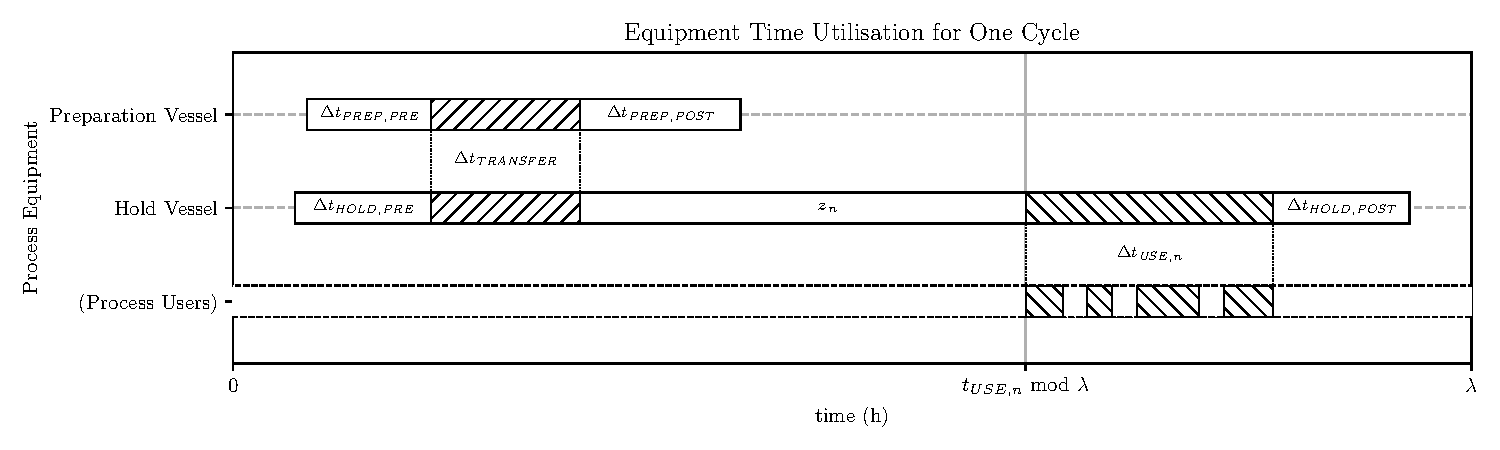
\includegraphics[angle=0,scale=0.55]{./figures/explanatory.pdf}
    \caption{Equipment time utilisation for a single buffer}
    \label{fig.explanatory}
\end{figure}

In addition to the buffer-specific and vessel-specific data detailed above,
some global parameters are required to specify the problem.
For the large-scale example, these parameters are tabulated in
\hyperref[tbl.parameters]{Table \ref*{tbl.parameters}} and are described in
more detail hereafter.

\begin{table}[h!]
    \centering
    \caption{Global parameters for large-scale example}
    \label{tbl.parameters}
    \begin{tabular}{l | l | r | c}
        symbol & short description & value & unit\\ \hline
        $\lambda$ & process cycle time & 96.0 & h\\
        $\Delta t_{\mathit{PREP,PRE}}$ & prep pre duration & 11.0 & h\\
        $\Delta t_{\mathit{PREP,POST}}$ & prep post duration & 2.5 & h\\
        $\Delta t_{\mathit{TRANSFER}}$ & transfer duration & 2.2 & h\\
        $\Delta t_{\mathit{HOLD,PRE}}$ & hold pre duration & 9.0 & h\\
        $\Delta t_{\mathit{HOLD,POST}}$ & hold post duration & 1.0 & h\\
        $\Delta t_{\mathit{HOLD,MIN}}$ & minimum hold duration & 12.0 & h\\
        $\Delta t_{\mathit{HOLD,MAX}}$ & maximum hold duration & 60.0 & h\\
        $r_{\mathit{MINFILL}}$ & minimum fill ratio & 0.27 & --\\
        $r_{\mathit{UTIL}}$ & maximum utilisation ratio & 0.7 & --\\
    \end{tabular}
\end{table}

The first parameter sepcified is the cycle time, $\lambda$.  We are concerned
with the steady-state operation of the process, so the cycle time can be
thought of as the duration from some fixed point in one batch to the same
fixed point in the subsequent batch.
The cycle time is typically some multiple of 24 hours.
This is for reasons of operability; it is easier for staff if a given task
occurs at the same time of the day for each batch.

In the model, the preparation and hold procedures are both broken into a number
of operations.
The durations of most of these operations are specified as global parameters.
It is unlikely that detailed timings will be available at the early stages of
design, so specifying some conservative global parameters provides a model that
is easy to comprehend and validate.
In reality, operations such as filling a vessel with water will scale with
buffer bolume and operations such as cooldown of a vessel after steaming will
scale with vessel volume.
This degree of granularity could be added as a future model enhancement.

The following durations are specified as global parameters:

The parameter $\Delta t_{\mathit{PREP,PRE}}$ is the duration of all operations
in the preparation procedure prior to the transfer of buffer to the buffer hold
vessel.  
This may include pressure testing, steam-in-place (SIP) and cooldown, although
these tasks are not always carried out on preparation vessels.
The period will include the charging of WFI, the charging of other liquids
and/or solids, and time for mixing the buffer.
It may also include some time for sampling or testing and adjustment of the
buffer.

The parameter $\Delta t_{\mathit{PREP,POST}}$ is the duration of all operations
in the preparation procedure that take place after the transfer of the buffer
to the buffer hold vessel is complete.
This is typically just comprised of the clean-in-place (CIP) of the vessel.
CIP involves a separate piece of equipment, the CIP skid, which circulates
cleaning fluids (detergents and/or acids, bases) through the vessel and some of
its attached pipework.

The parameter $\Delta t_{\mathit{PREP,POST}}$ is the duration of the transfer
of buffer from the preparation vessel to the hold vessel, via a sterile filter.
Although this varies with the buffer volume, the relationship is not that
straightforward.
As buffer and vessel volumes increase, a change in pipe diameter or pump size
may be appropriate, giving large step changes to the transfer duration.
Accordingly, a conservative global parameter for transfer duration is
appropriate for early-stage design.

The parameter $\Delta t_{\mathit{HOLD,PRE}}$ is the duration of all operations
in the hold procedure prior to the commencement of receipt of buffer from the
preparation vessel.
This typically includes pressure testing, SIP and cooldown.

The parameter $\Delta t_{\mathit{HOLD,POST}}$ is the duration of all operations
in the hold procedure that take place after the last use of buffer by the
process is complete.
Like $\Delta t_{\mathit{PREP,POST}}$, this is primarily comprised of a CIP of
the respective vessel.

Looking at the explanatory equipment time utilisation diagram, the one
parameter not yet mentioned is the buffer hold duration, $\boldsymbol{z}_{n}$.
Note that this is a decision variable, and not a parameter; it is discussed in
more detail in the subsequent chapter.
The buffer hold duration is the duration that spans from the end of the
transfer into the buffer hold vessel until the start of the first use of the
buffer by the process.
As will be described in the next chapter, we place some bounds on this duration
and express these bounds as a pair of global parameters.
The parameter $\Delta t_{\mathit{HOLD,MIN}}$ defines the minimum allowabe
duration of the buffer hold operation.
In practice, the operators of a plant do not want to schedule buffer
preparations so that the transfer is complete moments before the buffer is
required by the process, as any delays at this stage could imapct production.
A value, typically in the range of several hours to one day, can be specified
to ensure that buffers are prepared with some flexibility to handle delays.
At the other end of the scale, buffers may expire and the global variable 
$\Delta t_{\mathit{HOLD,MIN}}$ is defined to set a maximum allowable hold
duration.

When selecting a vessel, as mentioned in Section ???, a minimum fill ratio,
$r_{\mathit{MINFILL}}$ is defined to ensure that a vessel isn't selected that
is far too big for the buffer being prepared.

Finally, the utilisation ratio, $r_{\mathit{UTIL}}$, places an upper limit on
how busy a preparation vessel is allowed to be.
In the absence of detailed buffer scheduling information, this may represent an
`engineering factor' to account for unforseeable scheduling clashes.
If detailed scheduling information is available, the ratio can be set to unity
to effectively remove its influence as a constraint, or the ratio could be
maintained at some value to allow for some overhead in the design.

\section{Output Data}\label{S.outputdata}

This section describes the format of the outputs generated by the model, rather
than the values of the results themselves, which are discussed in detail in 
\hyperref[C.results]{Chapter \ref*{C.results}}.

The primary aim is to generate a list of the required preparation volumes.
For the example used in this chapter, the following table of results may be
generated.

\begin{table}[h!]
    \centering
    \caption{Required preparation vessels for large-scale example}
    \label{tbl.reqvessels}
    \begin{tabular}{r}
        vessel size\\ \hline
        \SI{8000}{\litre}\\
        \SI{10000}{\litre}\\
        \SI{15000}{\litre}\\
        \SI{20000}{\litre}\\
    \end{tabular}
\end{table}

While the above table gives the essential information allowing the buffer
preparation area to be sized and costed, it may be more instructive to return
a matrix showing where each buffer is to be prepared.
Such a matrix is shown in the table below.

\begin{table}[h!]
    \centering
    \caption{Buffer / vessel matrix for large-scale example}
    \label{tbl.bvmatrix}
    \begin{tabular}{l | c | c | c | c }
        & \SI{8000}{\litre} & \SI{10000}{\litre} & \SI{15000}{\litre} &
        \SI{20000}{\litre}\\ \hline
        Buffer \#1  &   &   &   & * \\
        Buffer \#2  &   &   &   & * \\
        Buffer \#3  &   &   &   & * \\
        Buffer \#4  &   &   & * &   \\
        Buffer \#5  &   &   &   & * \\
        Buffer \#6  &   &   & * &   \\
        Buffer \#7  &   & * &   &   \\
        Buffer \#8  &   &   & * &   \\
        Buffer \#9  & * &   &   &   \\
        Buffer \#10 & * &   &   &   \\
        Buffer \#11 & * &   &   &   \\
        Buffer \#12 &   &   &   &   \\
    \end{tabular}
\end{table}

Note that it is unlikely that there may exist more than one possible optimal
version of table xxx, especially if costs were scaled non-lineraly with vessel
volumes.
For the table above, many optimal version may exist; e.g. it may be possible to
switch the vessels in which buffers are prepared and still end up with the same
optimal vessel selection.
This phenomenon is dealt with in more detail in Section xxx.

While the above succinct table does give more information, it still doesn't
visibly confirm to the reader that the solution is feasible.
An equipment time utilisation plot provides a clear visual illustration of a
solution and displays a feasible schedule.
The explanatory plot in Figure xxx is an example of an equipment time
utilisation plot.  
An equipment time utilisation plot for the large-scale example covered in this
chapter is displayed below.
\begin{figure}
    \centering
    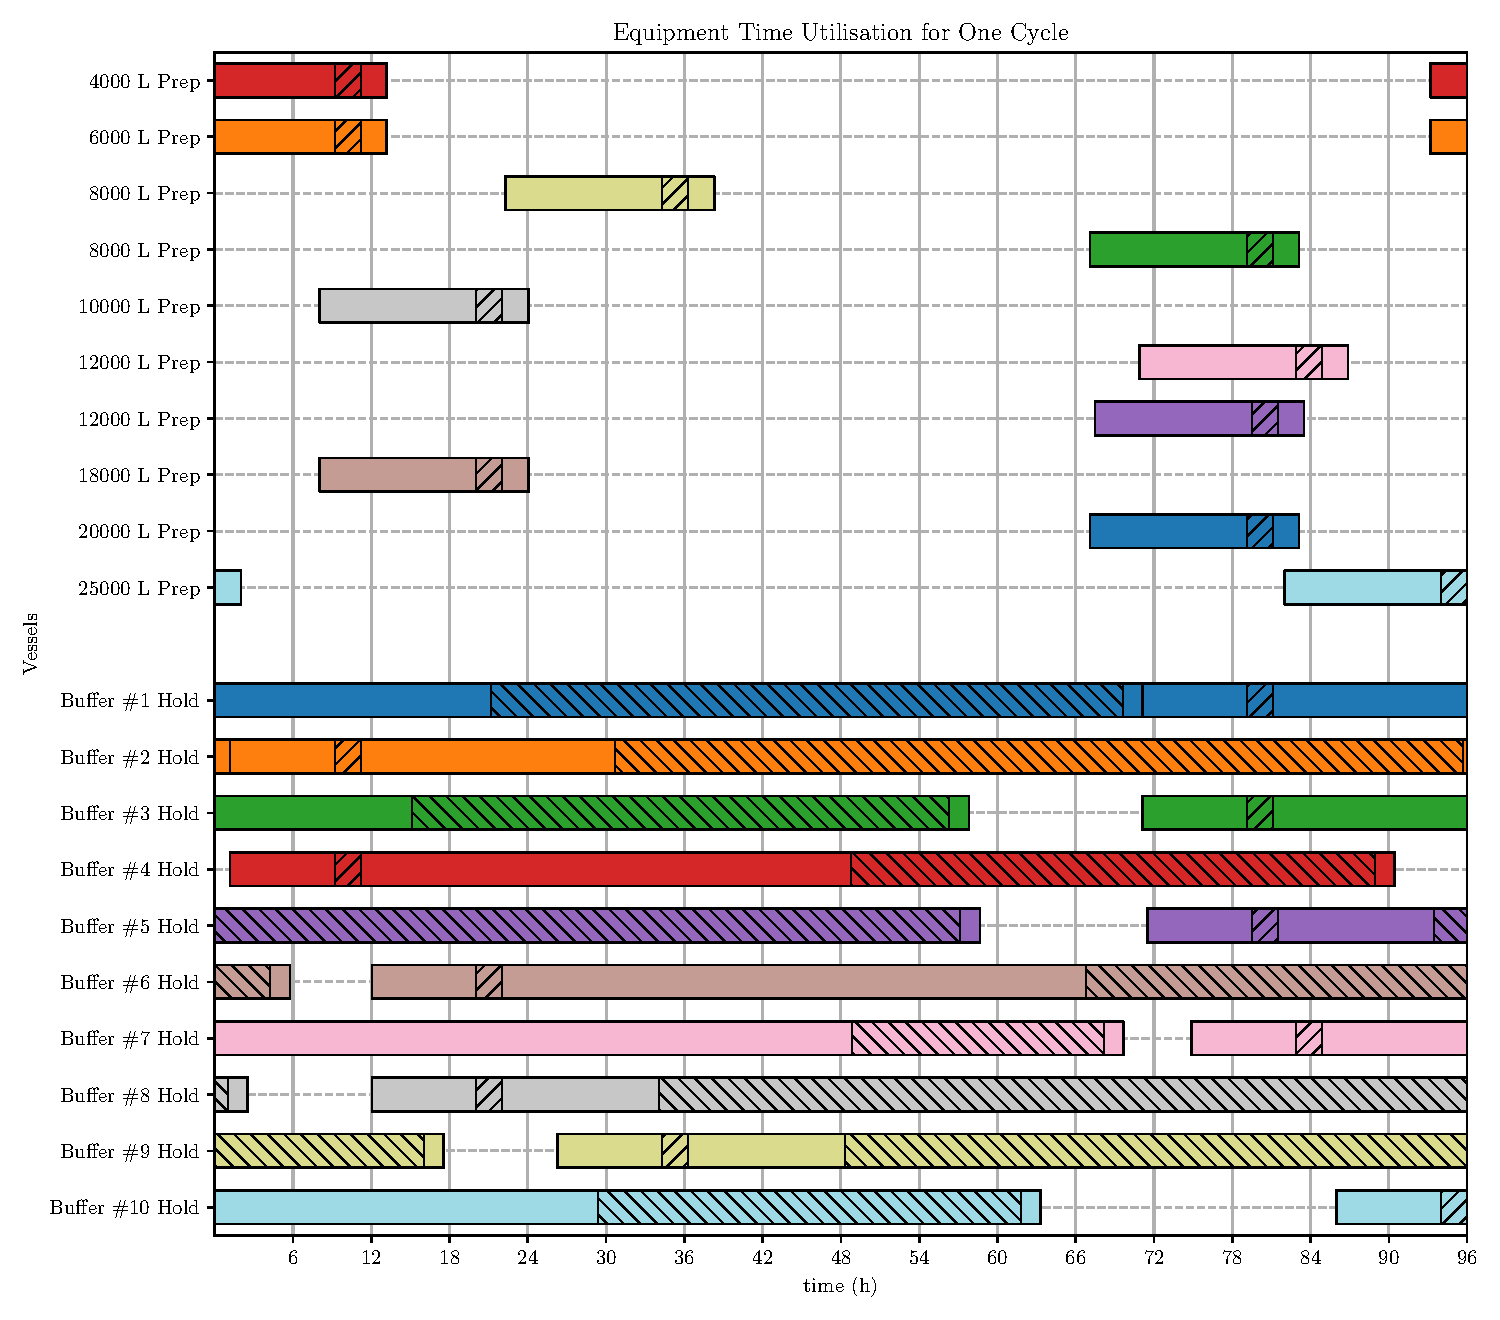
\includegraphics[angle=0,scale=0.55]{../examples/large-scale/plot1.pdf}
    \caption{Equipment time utilisation for large-scale example}
    \label{fig.etu1}
\end{figure}
Each horizontal entry represents a piece of equipment (preparation or hold
vessels in this case).
The presence of a bar indicates that the respective piece of equipment is in
use.  
The hatched bars indicate transfers, with backslash hatching representing the
transfer from the buffer preparation vessel to the buffer hold vessel and
forward-slash hatching representing the transfer of buffer from the hold vessel
to the process.
The latter is shown as a contiguous bar in the hold vessel, representing the
period from the start of the first use to the end of the last use of the buffer
in a given batch, although the demand from the process may be discontinuous.

Note that the time window shown in the plot is of a single cycle at
steady-state; the next cycle and the previous cycle would be identical.
In a sense, the offest of the single-cycle window is somewhat arbitrary; the
plot can be thought of as a cylinder that has been cut at right angles to its
ends and flattened out.
As it happens, for the buffers shown, none of their hold procedures start and
finish in the same cycle; they all overlap the cycle boundaries.

It should be noted also that the plot does not highlight which batches the
procedures belong to.
The entire downstream process may take more than one cycle to complete, so the
window visible in the plot could be showing buffer preparation and hold
procedures from several succesive batches.
